\chapter{Training}

\section{Loading the preprocessed data}

After processing the document into a standard and consistent from as discussed in chapter \ref{text_normalization}. the normalized form data can be stored in any database for frequently accessing the data for training purpose. In this experiment, the database used is Elastic Search. The author initially trained the classification model with only one feature ``Product name'' and the target being the lowest level of category.
Table \ref{table:AfterNormal} displays the difference in the number of records after removing the duplicate records on the normalized text. An Index in elastic search is a logical namespace for storing data in JSON format. The indexer names ``english-taxonomy-all'' contains the data before normalization. ``english-taxonomy-normal'' contains the data after normalization and removing the duplicate entries.

\begin{table}[H]
    \centering
    \caption{Record count before and after normalization}
    \label{table:AfterNormal}
    \begin{tabular}{ lll }
          \toprule
          
          \textbf{Index}& \textbf{Features} & \textbf{Count}\\
          \midrule
          english-taxonomy-all&Product name, Category & 22160\\
          english-taxonomy-normal&Product name, Category & 1507\\
          
          \bottomrule
          \end{tabular}
\end{table}

Pandas data frame \parencite{mckinney-proc-scipy-2010} provides the \textit{drop\_duplicates()} method to remove duplicate entries in the document. Code snippet in listing \ref{code:nt} has two methods ``normalize'' and ``clean''. In Pandas \parencite{mckinney-proc-scipy-2010}, ``apply'' method executes a function along a specified axis of data frame. Here for every text in the document of data frame variable ``df\_eng'', the method ``normalize'' is called to process the data. ``normalize'' function excepts a ``document'' as a parameter.  These texts are processed to remove any html tags using Beautiful Soup a python library. Using regular expression library the digits in between the characters are removed, white spaces are removed. Any special character within the text has been transformed to its normal form.

\clearpage

\begin{lstlisting}[language=Python,caption={Function to normalize text and remove duplicate},label={code:nt}]
    def clean(self):

        self.df_eng["name"]	= self.df_eng["name"].str.lower().apply(lambda n:self.normalize(n)) 
        self.df_eng["category"]	= self.df_eng["category"].str.lower().apply(lambda c:self.normalize(c))
        self.df_eng=self.df_eng.drop_duplicates()
       
    
    def normalize(self,doc):

        # Remove html tags 
        if doc:
            soup = BeautifulSoup(doc, 'html.parser')
            text =soup.get_text()
            text = (re.sub('[-\W]+', ' ', text))
            text = (re.sub('(?<=\d) (?=\d)', '', text))
            text = (re.sub("([a-z]\d+)|(\d+)", '', text))
            
            
            return ''.join(
            c for c in unicodedata.normalize('NFD', text)
            if unicodedata.category(c) != 'Mn')
      
\end{lstlisting}

\section{Fetch normalized data}
The normalized document is indexed in Elastic search analytic tool. In Elastic Search, the ``search'' function allows querying and retrieving data from indexed document. Code snippet in listing \ref{code:fndfes} fetches the indexed document. 

\begin{lstlisting}[language=Python,caption={Fetch normalized data from Elastic search},label={code:fndfes}]
    def getNormal(self):
        self.df_en = pd.DataFrame(columns=['name','category'])
        resp=self.es.search("english-taxonomy-normal",{"_source":["name","category"],                                  'size' : 5000,
        "query": {"match_all": {}}})
        for hit in resp['hits']['hits']:
                list_row_en = dict (name=None,category=None)            
                list_row_en["name"]=hit['_source']['name']             
                list_row_en["category"]=hit['_source']['category']
                new_row = pd.Series(list_row_en)
                self.df_en=pd.concat([self.df_en, new_row.to_frame().T], ignore_index=True)
        
        return self.df_en
      
\end{lstlisting}
\section{Train class initialization}
As illustrated in code listing \ref{code:ootc}, the class Train is instantiated by passing the normalized form of data. This is the data that will be used for training the machine learning model.
\begin{lstlisting}[language=Python,caption={Object of the Train class},label={code:ootc}]
    df_en = df.getNormal()
    train = Train(df_en)
\end{lstlisting}

\clearpage

\begin{lstlisting}[language=Python,caption={Train class constructor},label={code:tcc}]
from sklearn.feature_extraction.text import CountVectorizer
class Train():
    def __init__(self,df_en):

        self.vectorizer = CountVectorizer(1,1)
        self.df_en = df_en
        self.df_category = self.df_en.groupby("category")
        self.all_category = list(self.df_category.groups.keys())
        self.vectorizer.fit(doc=df_en["name"])
        self.inputSize=len(self.vectorizer.vocabulary_)
        self.n_categories=len(self.all_category)
        self.n_hidden = 128*3
        self.rnn= RNN(self.inputSize, self.n_hidden, self.n_categorie)
        self.learning_rate=0.005
        self.criterion = nn.NLLLoss()
        self.current_loss = 0
        self.all_losses = []
\end{lstlisting}

The code snippet listing \ref{code:tcc} shows the initialization of \textit{Train} class attributes. Code listing \ref{code:tcc} describes the  initialization the required attributes qualifying the building blocks of a neural network, such as object of class \textit{RNN} defining the input size, number of hidden layers, and size of the output. The loss function $L$, learning rate $l$, training dataset containing the true labels $y_{true}$ are initialized.

\begin{enumerate}
    \item self.vectorizer : Is an instance of \textbf{CountVectorizer} from scikit-learn \parencite{sklearn_api}. The details of Count vectorization is in section \ref {ch_countvector}.  The argument (1,1) indicates that the vectorizer will consider individual words as the vocabulary.
    \item self.df\_category: Stores the categorical classification of input data df\_en
    \item self.all\_category : This attribute is created to store all unique categories found in the category column of the input df\_en.
    \item self.vectorizer.fit(doc=df\_en[``name"]): The fit method of the vectorizer is called on ``name'' column of input data ``df\_en'' to build the vocabulary and transform text data in to numerical representation.
    \item self.inputSize : It sets the input size of the neural network to the size of the vocabulary.
    \item self.rnn: \acl{RNN} is initialized with updated input size, and number of hidden units and the number of unique categories as the output size.
    \item self.criterion: An instance of \acf{NLLLoss} pytorch function is stored. The function to minimize or maximize is called the objective function, or criterion \parencite[Section 4.3]{Goodfellow-et-al-2016}.
    \item self.all\_losses and self.current\_loss: These attributes are used to track the loss values during the training process.
\end{enumerate}

\clearpage

\section{Fetch Training Dataset}

The code listing \ref{code:rtcc} defines a method ``randomTrainingExample''. This method is responsible for generating training examples that will be used during the training process of the neural network. This function fetches the pair of vectorized input $x^i$ that is the tensor representation of product name and true target label $y^i_{true}$ which is the tensor representation of category.

\begin{lstlisting}[language=Python,caption={Train class constructor},label={code:rtcc}]
def randomTrainingExample(self):
    
    randcategory = random.choice(self.all_category)
    # get feature name from the category
    random_feature_indices = self.df_category.indices[randcategory]
    
    index = random_feature_indices[random.randint(0, len(random_feature_indices) - 1)]

    name =self.df_en.iloc[index]["name"]
    
    category_tensor = torch.tensor([self.all_category.index(randcategory)], dtype=torch.long)
    
    name_tensor = self.helper.nameToTensor(name)
    
    return randcategory, name, category_tensor, name_tensor
\end{lstlisting}

\begin{itemize}
    \item randcategory = random.choice(self.all\_category) : This fetches random category from the list of categories extracted during the initialization of ``Train'' class  
    \item random\_feature\_indices = self.df\_category.indices[randcategory]: The indices of the randomly obtained category from step 1 is stored from the grouped dataframe ```df\_category'''
    \item index = random\_feature\_indices[random.randint(0, len(random\_feature\_indices) - 1)] :\\ Random index is obtained from the list of indices of data sample belonging to the selected category.
    \item name = self.df\_en.iloc[index]["name"]:\\ Name of the product is accessed from the ``name'' column of the data frame. It is accessed using randomly chosen index. It accesses the name (text data) associated with selected category.
    \item category\_tensor = torch.tensor([self.all\_category.index(randcategory)], dtype=torch.long : \\ A tensor is created to represent the index of the randomly selected category. This tensor will be used during training as the target label for the corresponding input "name\_tensor".
    \item name\_tensor = self.helper.nameToTensor(name): The product name is converted into a tensor with a custom defined ``helper'' class. Code listing \ref{productnametotensor} is defined within the helper class.
    

\end{itemize}

\clearpage

\section{Training Execution}

In code listing \ref{code:train_function} the \acl{NLLLoss} is calculated between the output of the \acf{RNN} $ y_{pred} $ which is the predicted-log-probabilities and the ground truth category tensor $y_true$.

\begin{lstlisting}[language=Python,caption={Train function},label={code:train_function}]
    
    def train(self,category_tensor, name_tensor):
        
        hidden = self.rnn.initHidden()
    
        self.rnn.zero_grad()
            
        output, hidden = self.rnn(name_tensor, hidden)
        loss = self.criterion(output, category_tensor)
        loss.backward()
       
        # Add parameters' gradients to their values, multiplied by learning rate
        for p in self.rnn.parameters():
            p.data.add_(p.grad.data, alpha=-self.learning_rate)
    
    
        return output, loss.item()
    \end{lstlisting}

\subsection{\acl{NLLLoss}} 
The negative log likelihood loss is useful to train a classification problem with ``C'' classes or target labels \parencite{Paszke.03122019}. These labels are integers representing class indices. The \acl{NLLLoss} is often used with $LogSoftMax$ activation function. In the final layer of the neural network, adding the 
$LogSoftMax$ functions return the predicted log-probabilities. The loss is calculated by comparing the predicted log probabilities with the true target labels $y_{true}$. 






\subsection{\acf{BPTT}}

Detailed explanation of back propagation is given in section \ref{sec:minloss}. \\ In code listing \ref{code:train_function} the loss.backward() method of the loss function performs back propagation. RNN is a computational graph with parameters holding memory of previous time step. A computational graph is a record of all data (tensors) and all executed operations in a \acf{DAG}. The leaves of a \acsp{DAG} are the input tensor, roots are the output tensors. Unrolling the computational graph and then applying the back propagation algorithm is called \acl{BPTT} \parencite[section 15.2.5]{pml1Book}.

\subsection*{How the backward() method works?} \label{sec:backward}

\begin{enumerate}
    \item During forward propagation of \acs{RNN} module (refer section \ref{sec:math-rnn}) with output of $LogSoftMax$ activation function, the log probabilities computation operations are recorded along with the computational graphs.  
    \item The \textbf{backward()} on a scalar tensor start traversing the computational graph in reverse order (from \acs{DAG} root to leaves). For each step it applies chain rules of calculus flowing backward through the network in order to compute the gradients \parencite[section 6.5.2]{Goodfellow-et-al-2016}.

\end{enumerate}
\clearpage
\subsection{Model Parameter Optimization}
At line number 13 of code listing \ref{code:train_function}, the loop updates the model parameter.
\begin{itemize}
    \item  The gradients are accumulated in the Pytorchs  \textbf{torch.Tensor.grad} attributes of the input tensors. \footnote{https://pytorch.org/tutorials/beginner/blitz/autograd\_tutorial.html}
    \item These gradients can be accessed to update the model parameters through an optimization algorithm  like \acf{SGD} (refer chapter \ref{ch:math-behid} for more details).
    \item Iteratively trained neural network's  gradient-based optimizers drive the cost function($LogSoftmax$) to a very low value. 
\end{itemize}

\section{Experimentation: Variation in the training parameters.}

\subsection*{Training without \acs{BPTT}}

These are the observations when \textbf{loss.backward()} function in code listing \ref{code:train_function} is not used.

\begin{enumerate}
    \item Pytorch's tensor.grad value is None. Hence, the manual optimization step does not update the model parameters.
    \item Commenting the line number 9 and 10 from code listing \ref{code:train_function}, completes the training process. However, the model does not learn anything.  
    \item The figure \ref{fig:nograd} shows the loss across the training process. As the loss are not nearing to zero this shows that the model has failed in supervised learning of classification task.
    \begin{figure}[H]
        \centering    
        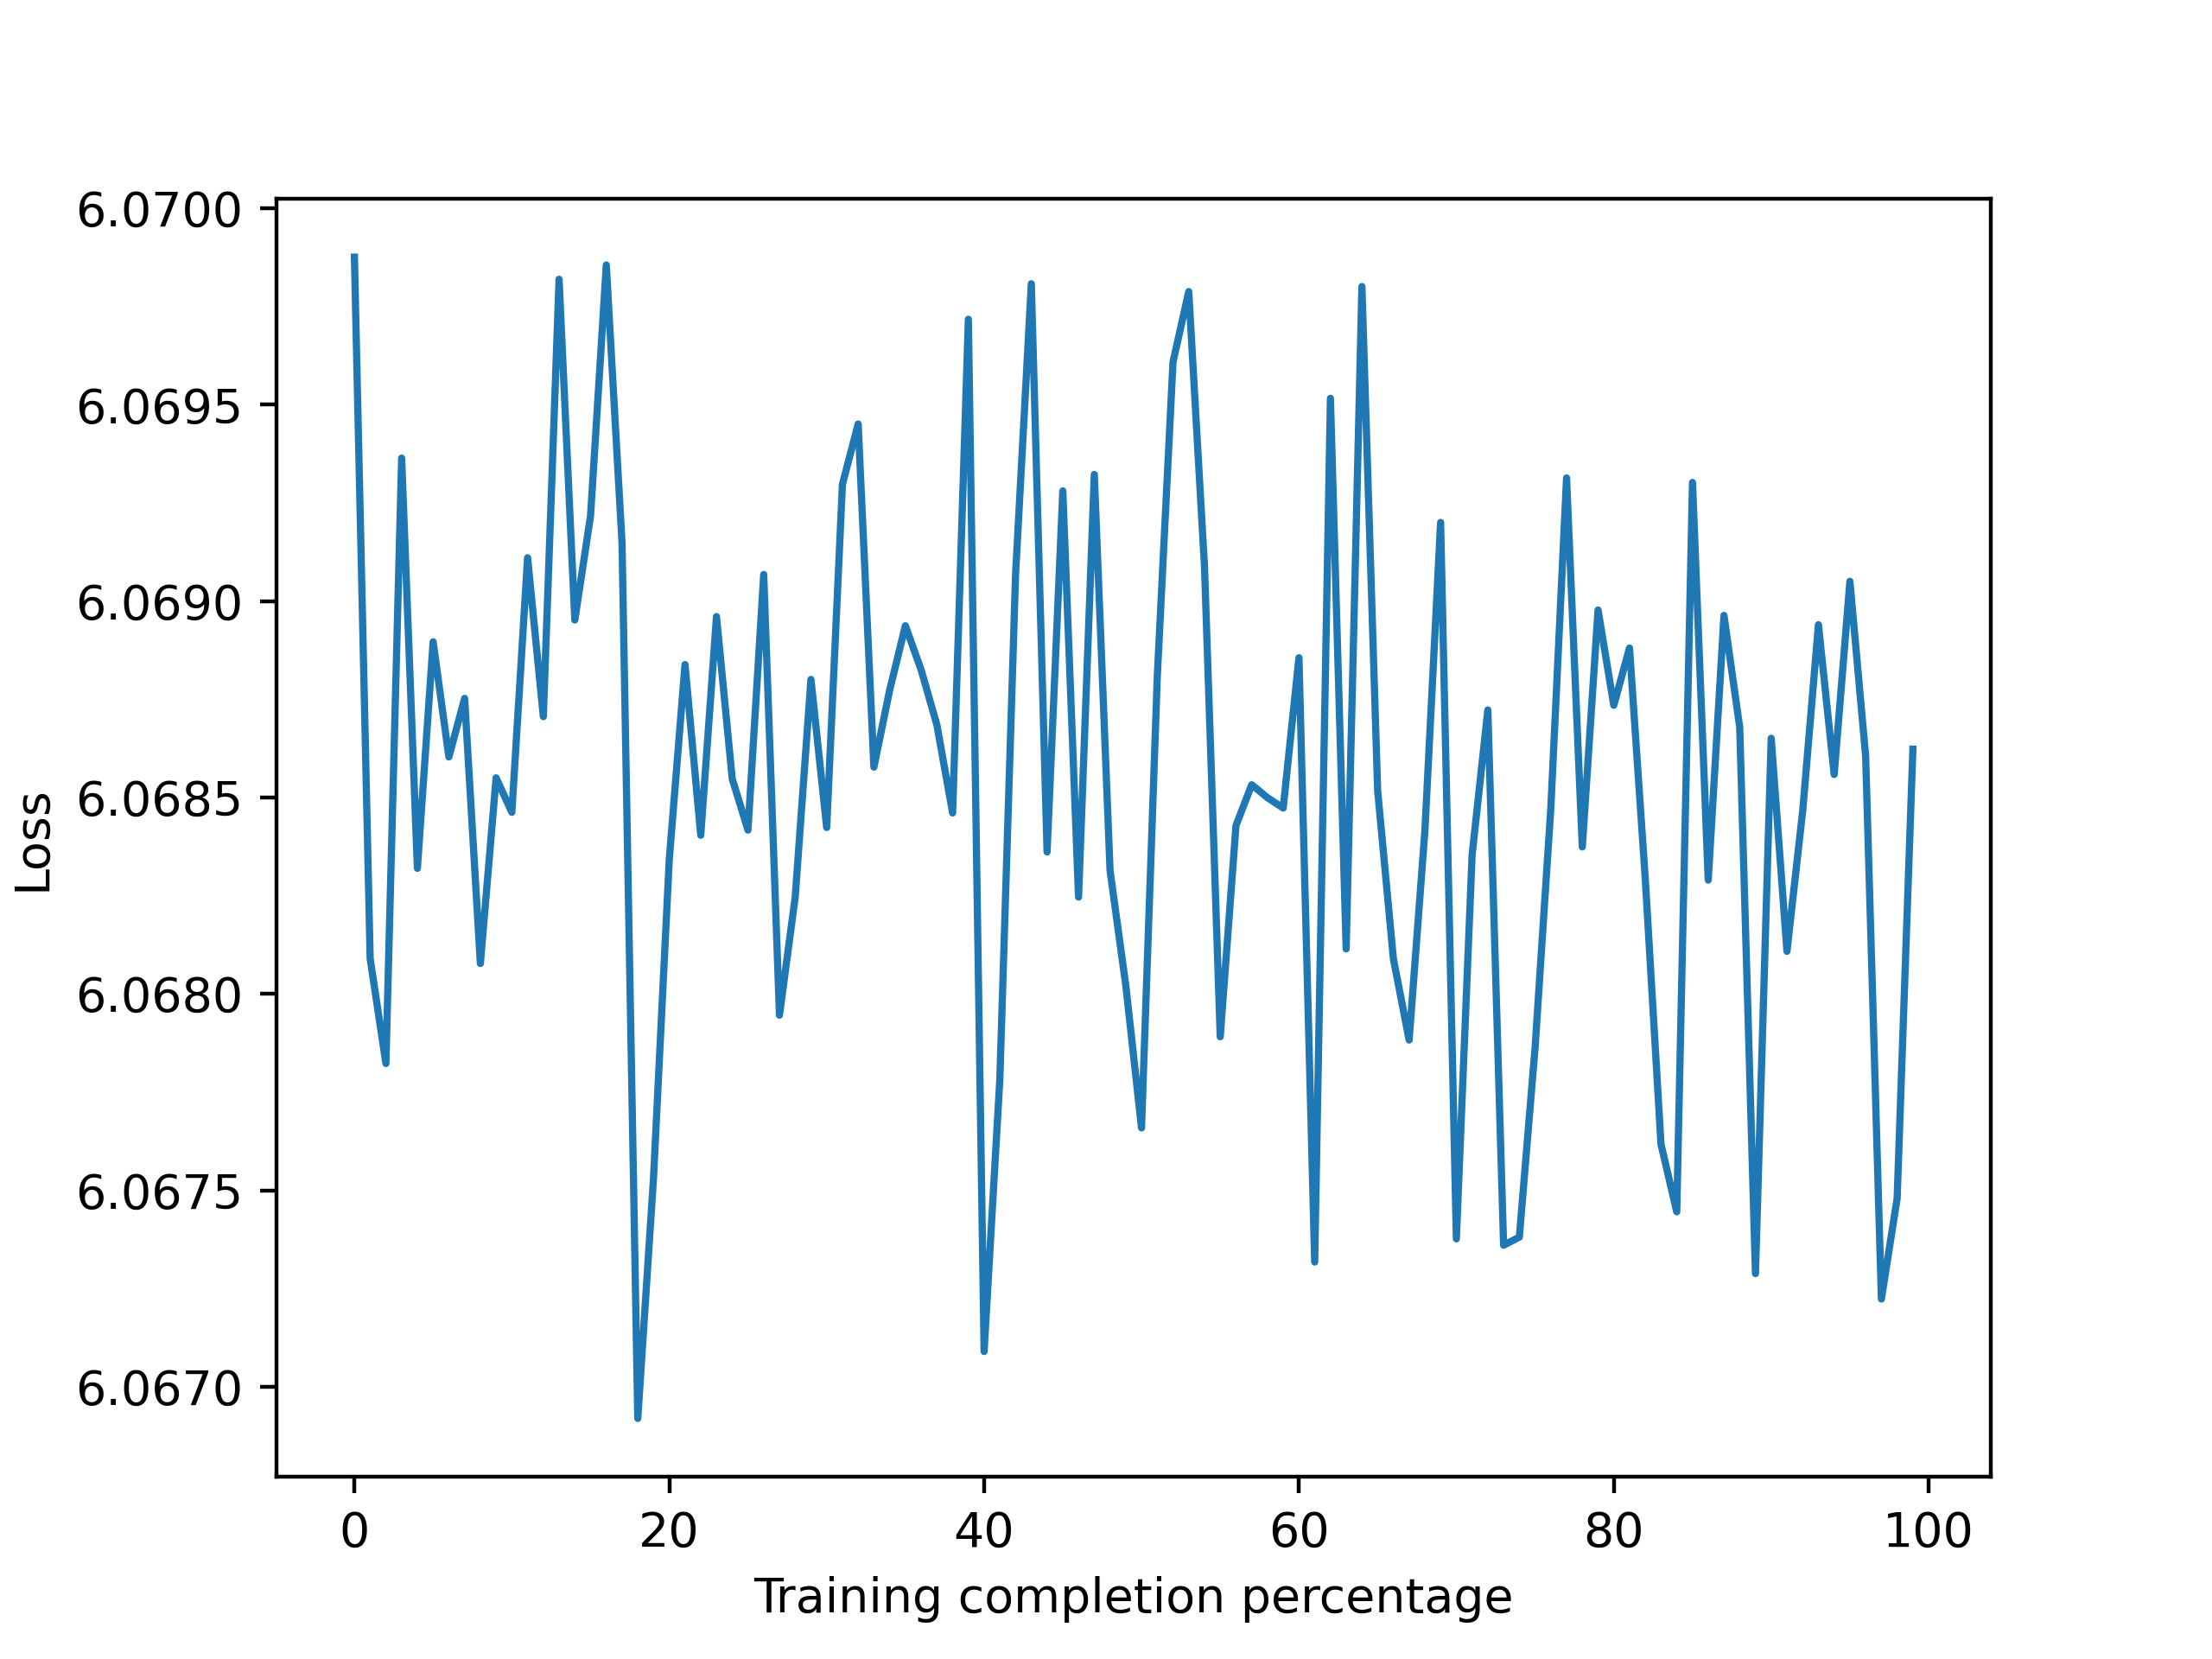
\includegraphics[scale=0.9]{loss_nograd.png}
        \caption{Loss without back propagation}
        \label{fig:nograd}
    \end{figure}
    
\end{enumerate}


\subsection*{Training without updating the model parameters}
In this experiment, the \textbf{loss.backward()} method calculated the gradients. However, the model parameters were not updated by commenting the line number 16 and 17 from code listing \ref{code:train_function}. Notice in the figure \ref{fig:nograd} and figure \ref{fig:womp}, the loss is not reaching zero towards the end of the training. Indicating that in both the cases the model has not learned the product name patterns for the classification task.

\begin{figure}[H]
    \centering    
    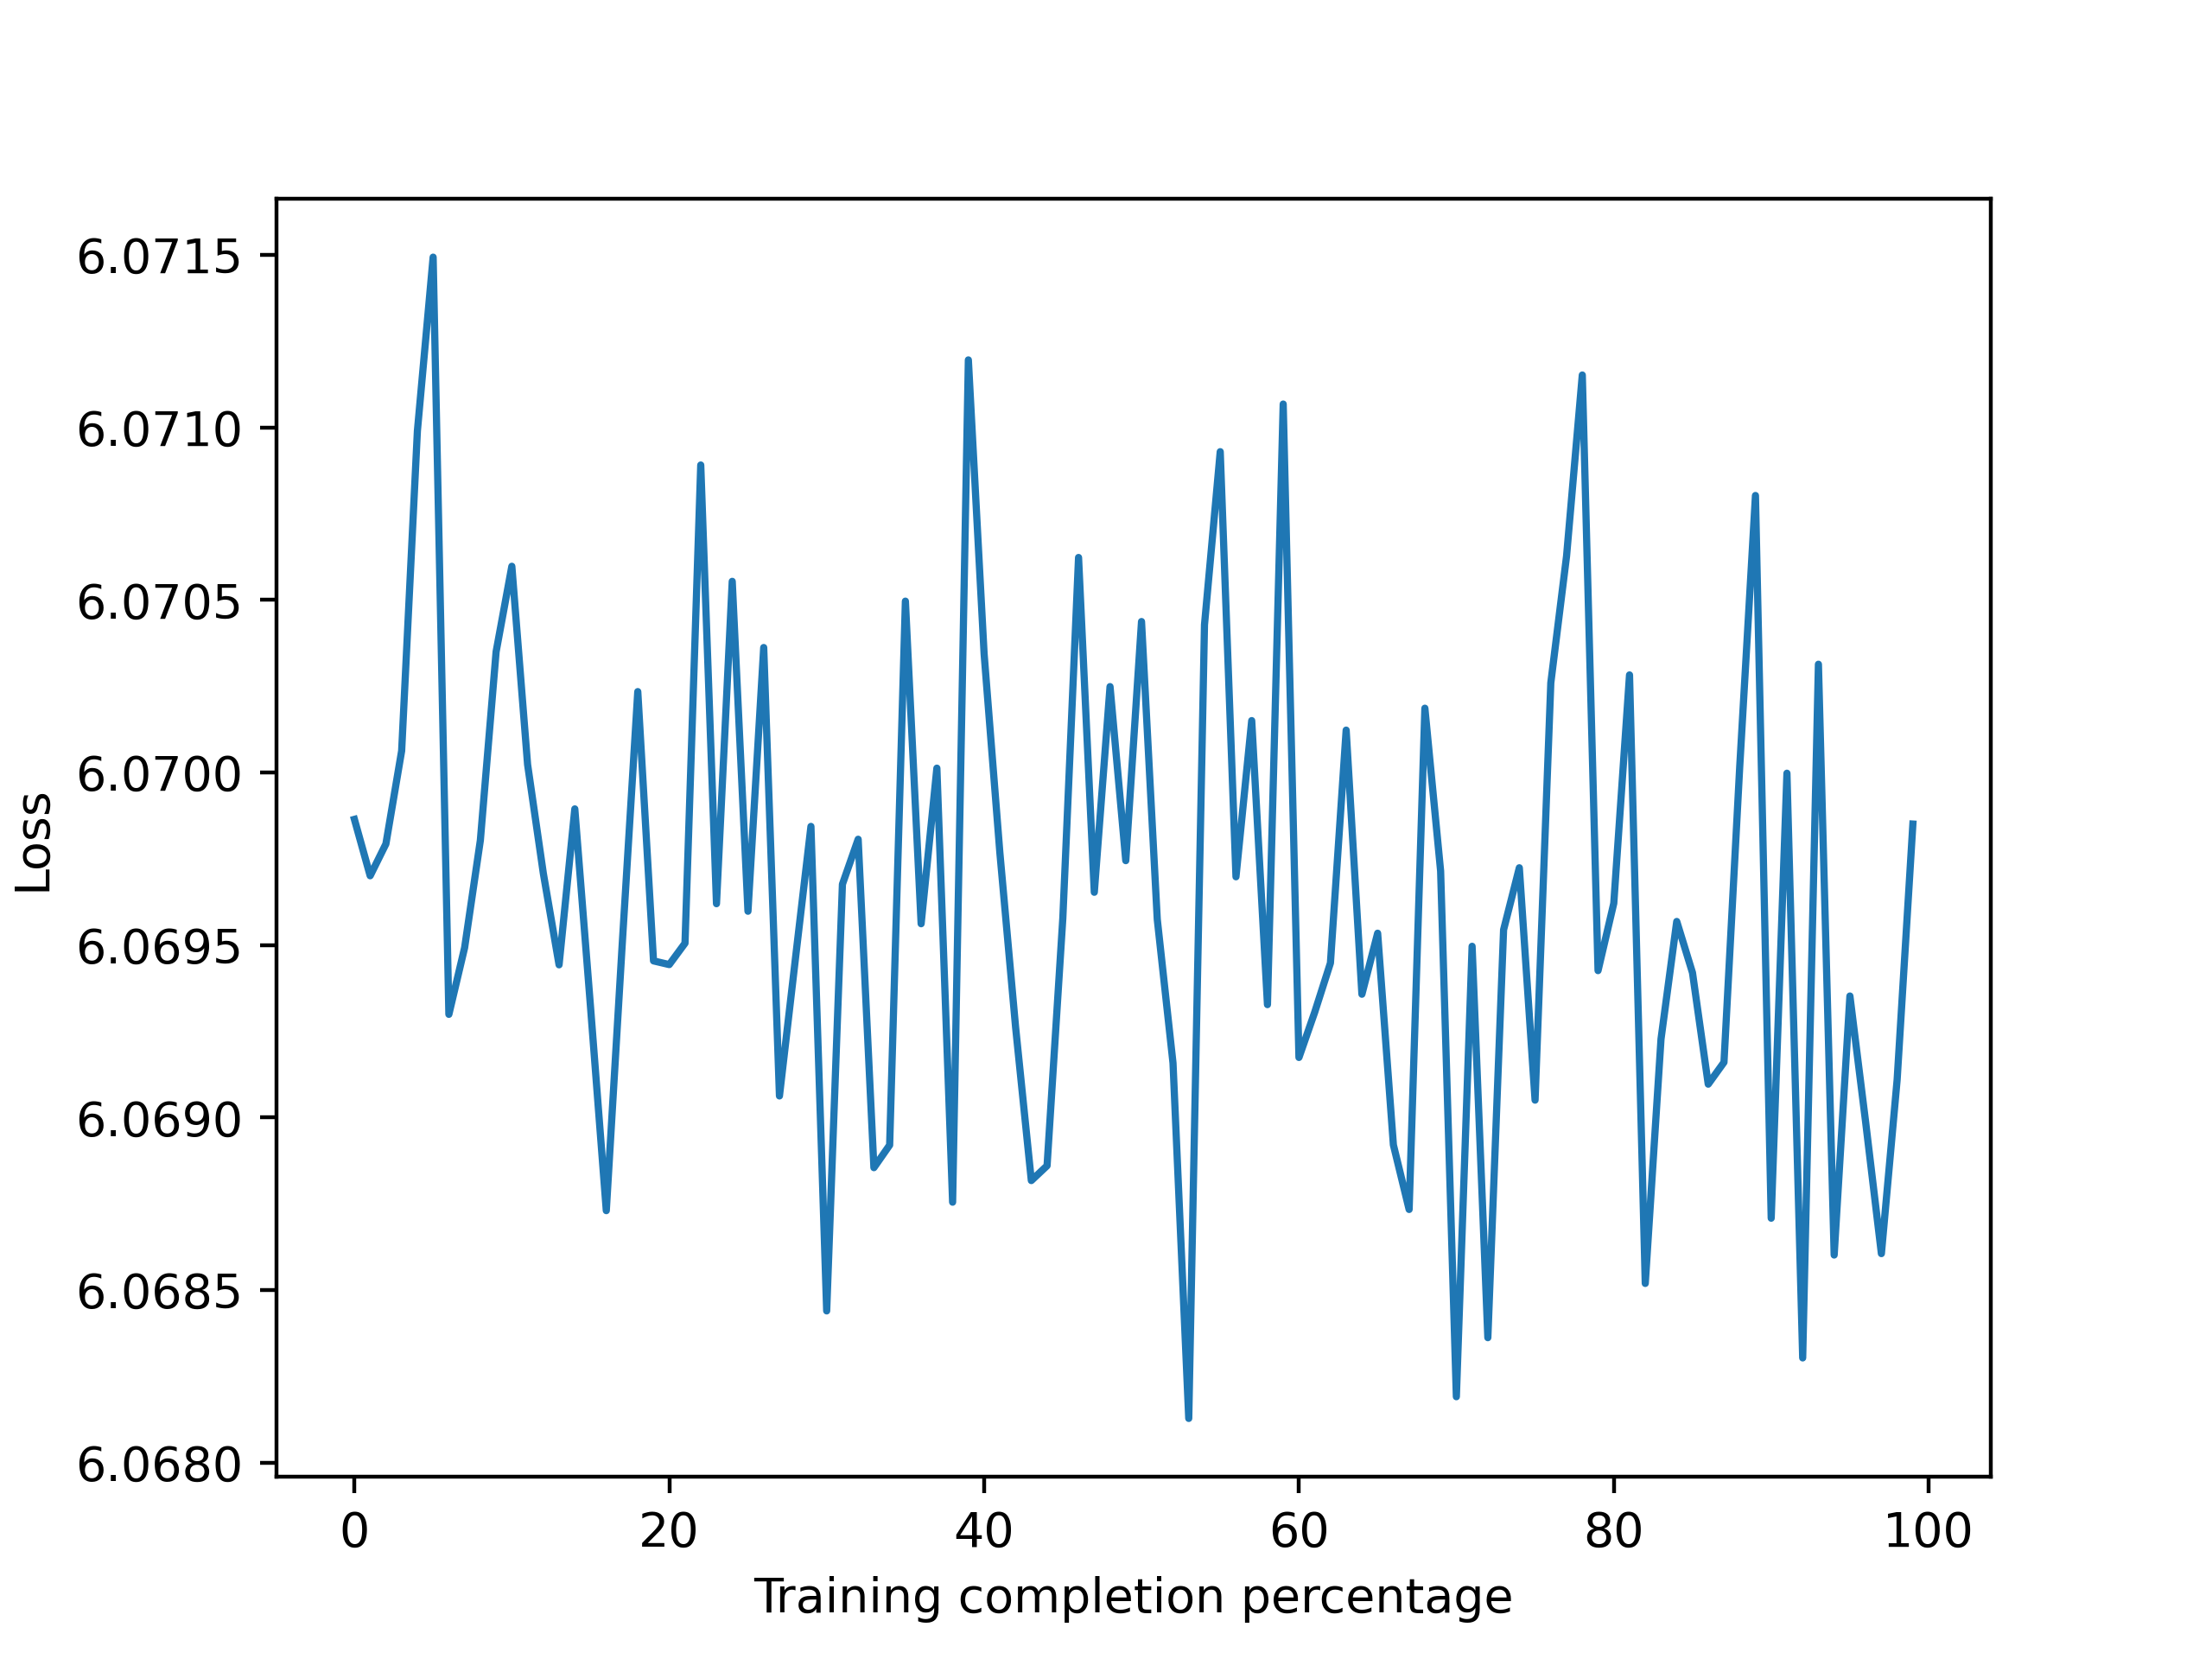
\includegraphics[scale=0.9]{loss_womp.png}
    \caption{Loss without updating the model parameters}
    \label{fig:womp}
\end{figure}

\subsection{Training with manually updating the model parameters} \label{sec:tmump}

The code listing \ref{code:mump} iterates through the parameters and updates their value based on the gradients computed during back propagation. 

\begin{lstlisting}[language=Python,caption={Manual gradient updation}, label={code:mump}]
    # Add parameters' gradients to their values, multiplied by learning rate
        for p in self.rnn.parameters():
            p.data.add_(p.grad.data, alpha=-self.learning_rate)
\end{lstlisting}

In code \ref{code:mump}, the parameter ``p.data'' is a tensor. The method  ``add\_()'' multiplies the argument and then add the product value to the tensor data ``p.data''. In this case, the negative value of ``learning\_rate'' is multiplied with the parameter gradient data and then the value is added to the ``p.data'' attribute.

\begin{figure}[H]
    \centering    
    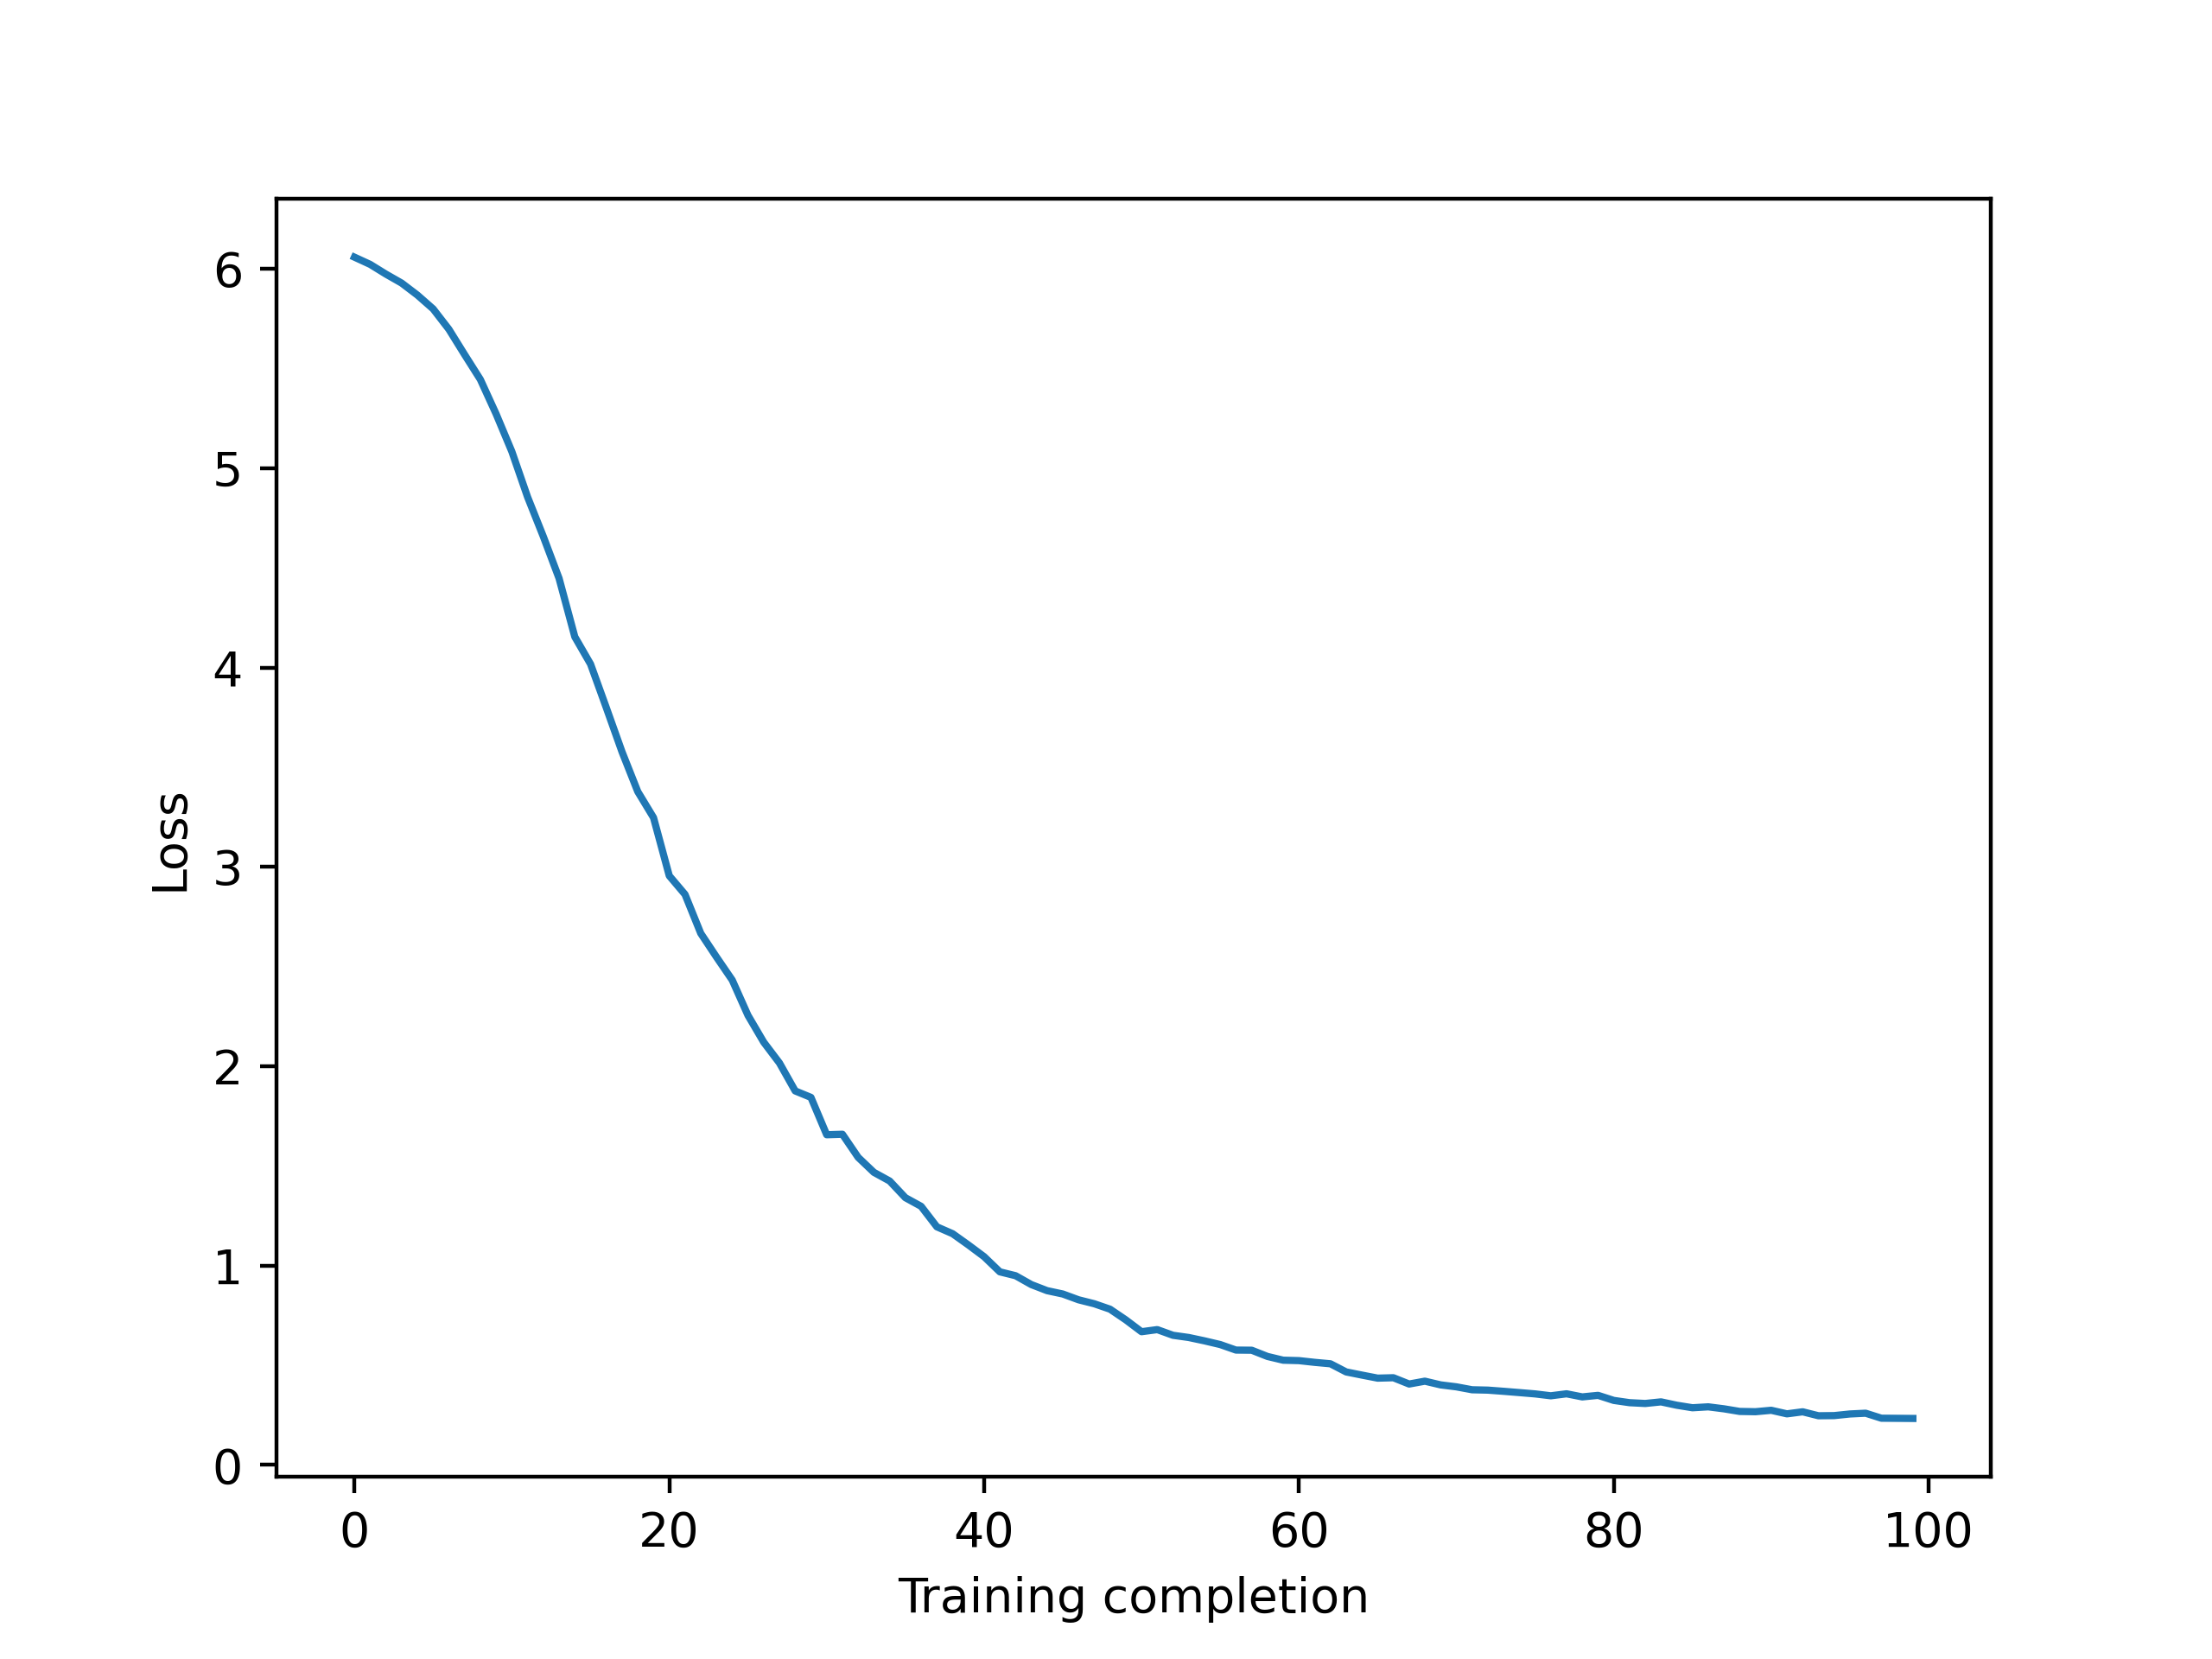
\includegraphics[scale=0.9]{loss_wmp.png}
    \caption{Loss with manually updating the model parameters with learning rate}
    \label{fig:wmp}
\end{figure}


\subsection*{Updating the hidden number of units}

The model is described as a \acl{DAG} describing how functions are composed together. Consider having three functions $f(x) = f_3(f_2(f_1(x)))$ connected in a chain. $f_1$ is the first layer of the network, $f_2$ the second and so on. In the example of a classifier, $y=f_*(x)$ maps an input $ x $ to a category $ y $. The final layer of the network is called the output layer. The training data specifies what the output layer must do at each point $x$, that is to produce a value close to $y$. As the training data does not show the desired output for other layers, they are called \textbf{hidden layers}  \parencite[Chapter 3]{Goodfellow-et-al-2016}.  \parencite{zhang2021dive} describes the concept of \textbf{hidden state} which are inputs at step $t$ can only be computed with previous input at step $ t-1 $. \acf{RNN} are neural network with hidden states.

\subsubsection*{Model with only one hidden state}
In this experiment, only one hidden state has been assigned to the \acs{RNN} network. As illustrated in figure \ref{fig:unihidden}, the loss reduces gradually. However, the model is yet under fit for the classification task. The loss not reaching zero towards the end of the training indicates that the model has not learned anything significant.

\begin{figure}[H]
    \centering    
    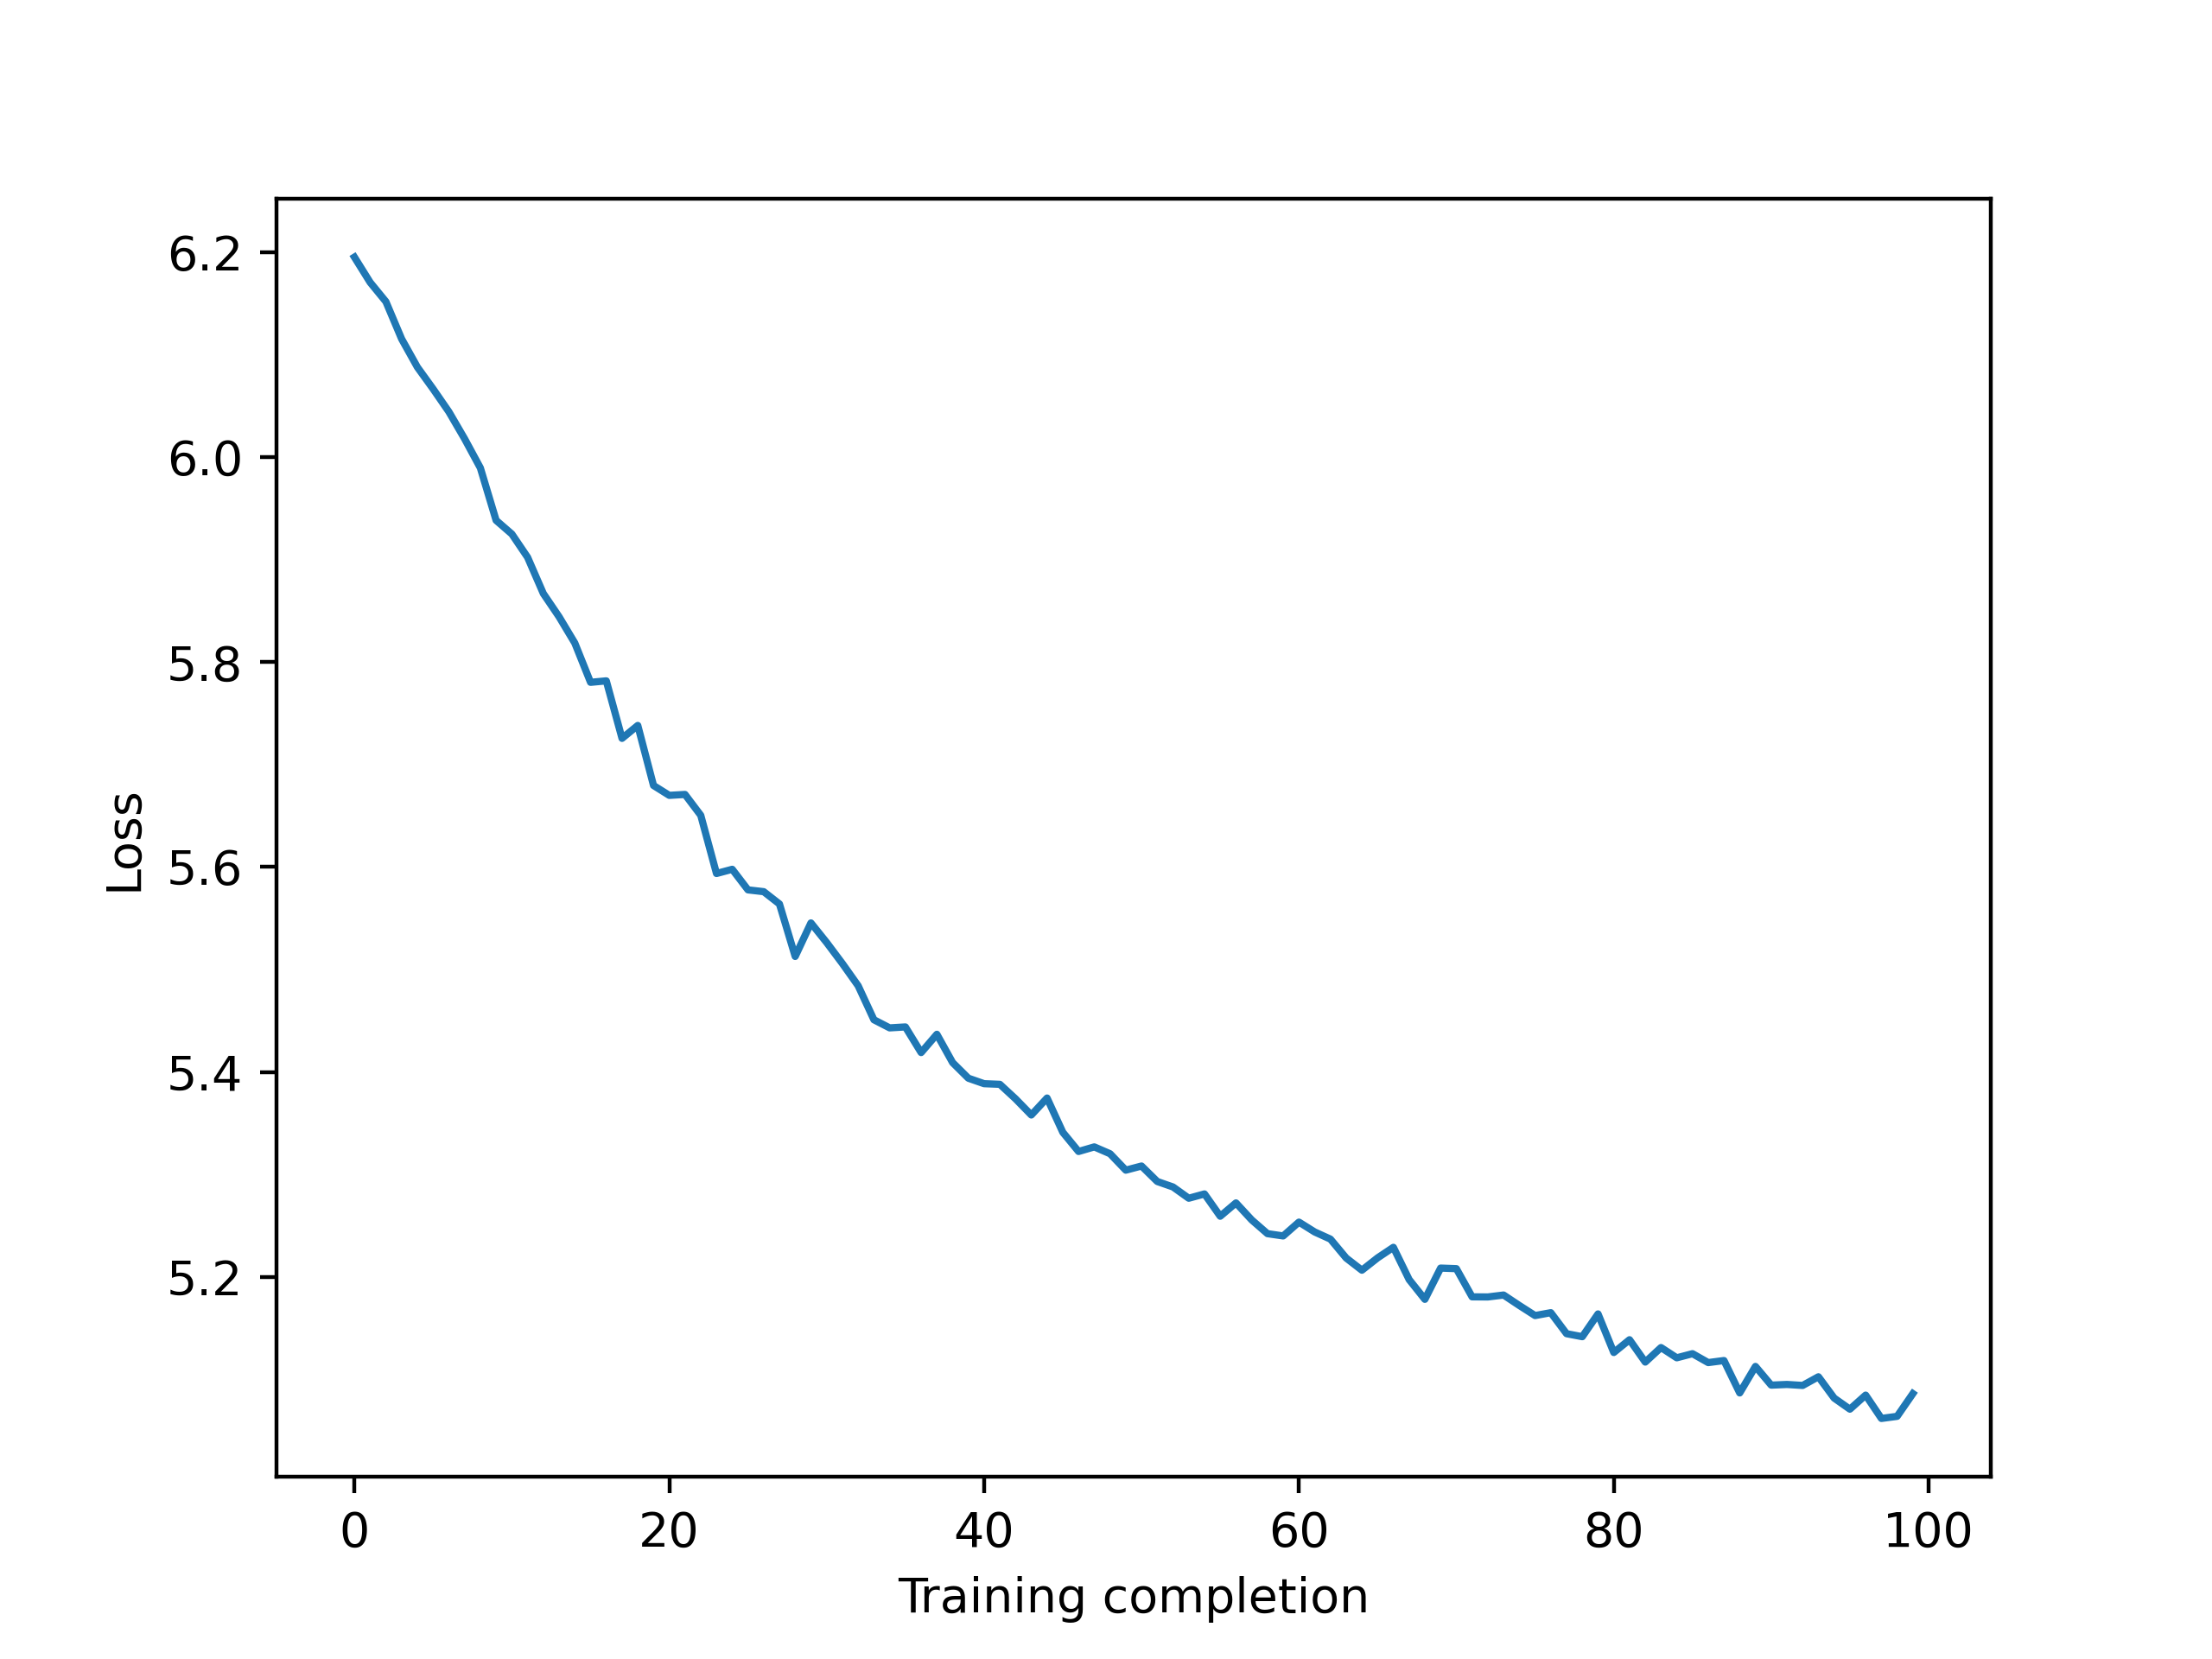
\includegraphics[scale=0.9]{loss_1hidden.png}
    \caption{Model with only one hidden state}
    \label{fig:unihidden}
\end{figure}

\subsubsection*{Model with only 10 hidden state}
Increasing the number of hidden state to 10 units gave the desired result.  As seen in figure \ref{fig:10hidden}, the loss has reached near zero by end of the training. This model is able to predict the category based on the pattern of name.
\begin{figure}[H]
    \centering    
    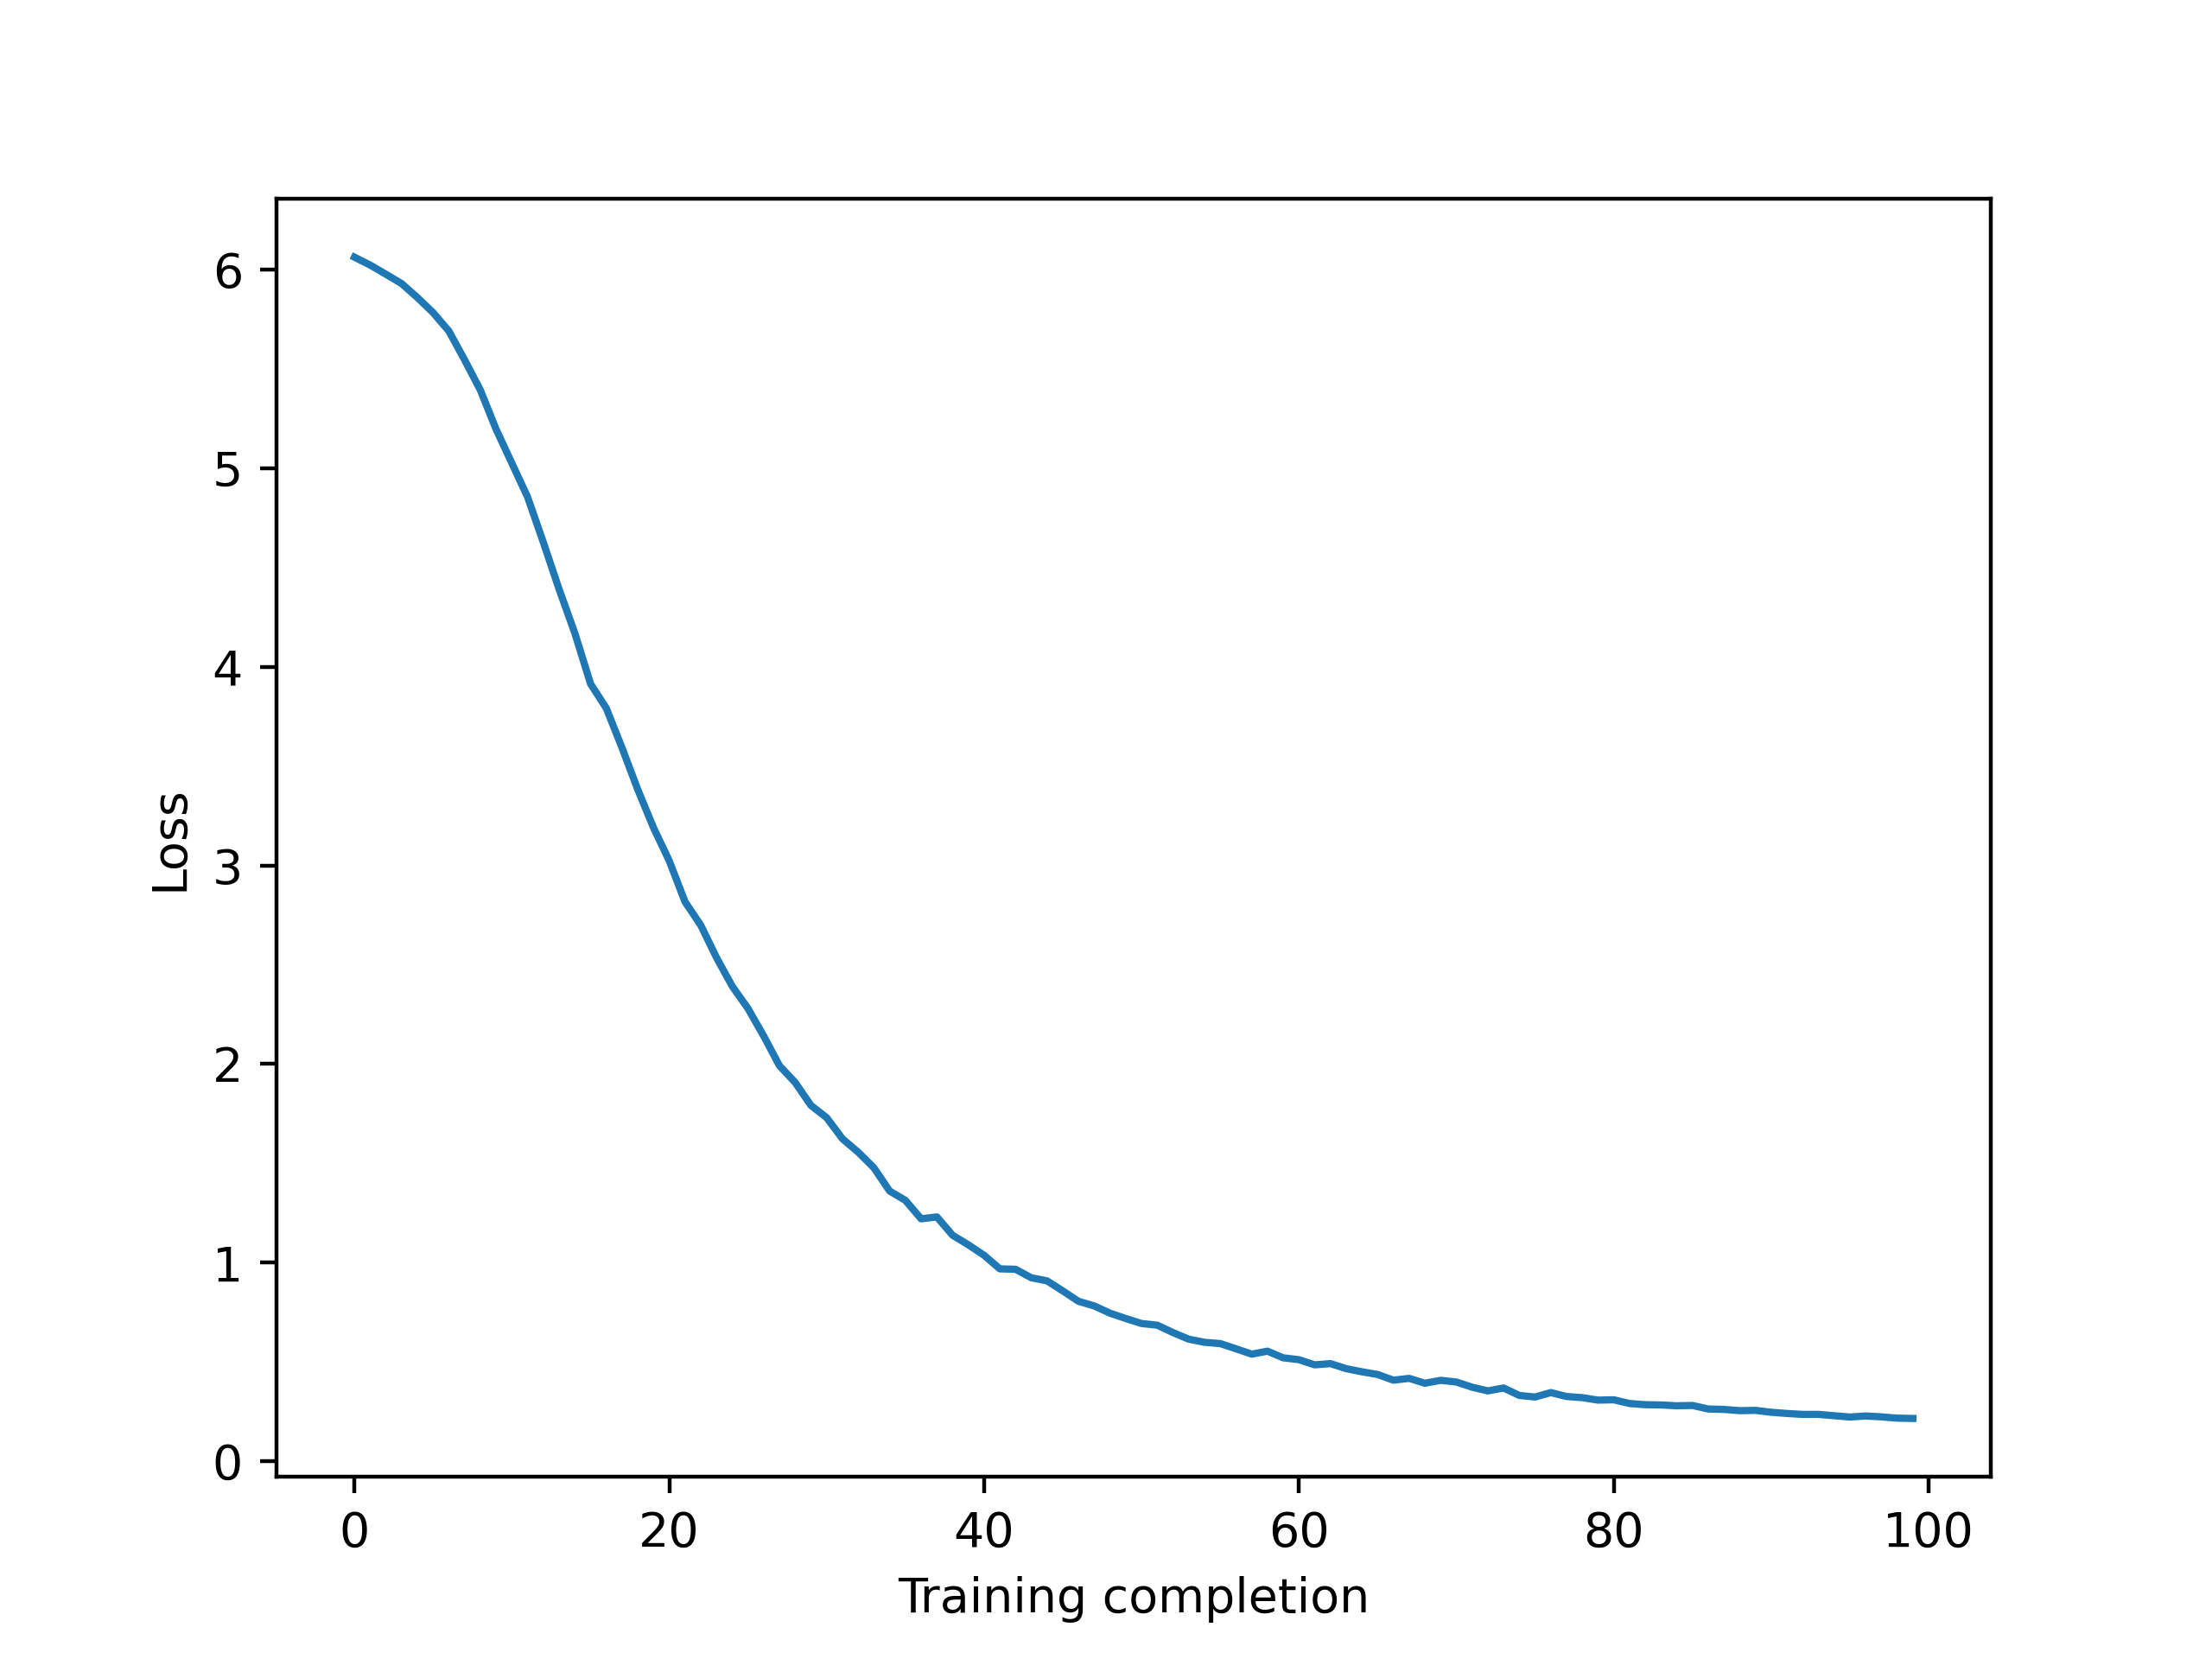
\includegraphics[scale=0.9]{loss_10h.png}
    \caption{Model with only 10 hidden state}
    \label{fig:10hidden}
\end{figure}

\section{Gradient decent step adjustment}

As stated in section \ref{sec:backward}, the method \textbf{loss.backward()} computes the gradients by applying chain rule of calculus for each function $f(x)$. The derivative of this function is denoted as $f'(x)$ \\ or as $\frac{dy}{dx}$. $f(x)$ can be reduced by moving $x$ in small with steps opposite sign of derivative is called gradient decent \parencite{cauchy}.  \parencite[section 4.3]{Goodfellow-et-al-2016} presents an equation \ref{eq:update_rule}.

\begin{align}
    x_i = x_i - \epsilon \frac{\partial}{\partial x_i} f(x) \label{eq:update_rule}
\end{align}

\begin{itemize}
    \item \( x_i \): The \(i\)th parameter of the model (weight or coefficient).
    \item \( \epsilon \): The learning rate, a positive scalar which determines the size of the step.
    \item \( f(x) \): The cost or loss function trying to minimize.
    \item \( \frac{\partial}{\partial x_i} f(x)\): The partial derivative  measures how \( f \) changes as only the variable \( x_i \) increases at point  \( x \).
\end{itemize}


In section \ref{sec:tmump}, refer to the code listing \ref{code:mump}, based on the equation \ref{eq:update_rule} we conclude that the variable \textit{p.grad.data} represents the partial derivative \( \frac{\partial}{\partial x_i} f(x) \) and the negative value of variable \textit{self.learninig\_rate} is included to subtract product of  variable \textit{p.grad.data} and variable \\ \textit{self.learninig\_rate} with variable \textit{p.data}. The same result can be achived by using pytorch's  \textit{subtract\_} method without negating the value of \textit{self.learninig\_rate}.

\begin{lstlisting}[language=Python,caption={Manual gradient updation with substract\_}, label={code:mumps}]
    # Add parameters' gradients to their values, multiplied by learning rate
        for p in self.rnn.parameters():
            p.data.subtract_(p.grad.data, alpha=self.learning_rate)
\end{lstlisting}

\section{\acf{CLR}}

Learning rate is an important parameter to tune the training of deep neural network. \parencite{Smith.03062015} describes a new method to set the learning rate called \acf{CLR}. In this method the learning rate in the training cyclically vary between the reasonable boundaries of the learning rate instead of having a fixed learning rate.

The steps involved in training a model with \acs{CLR} are as follows :

\begin{enumerate}
    \item Define the Learning rate range or reasonable boundary value: \\
    In this step, by linearly increasing the learning rate during training can specify the learning rate range in which an optimal accuracy is obtained. The lower point of range can be referred as $base\_lr$ and higher point as $max\_lr$.
    \item Training the model by gradually decreasing the learning rate to $base\_lr$ and again increasing the learning rate to $max\_lr$ over an interval of a constant step size.
\end{enumerate}


\subsection*{Experimentation and analysis to determine learning rate range}

\begin{enumerate}
    \item Experiment by setting $base\_lr$ and $max\_lr$  manually : \\
    In this experiment, the learning rate range is set manually to very low and high values. Numpy np.linspace() \parencite{harris2020array} returns the evenly spaced numbers between the  $base\_lr$ and $max\_lr$ over a specified interval.

    The result of training process the model with $base\_lr =1 \times 10^{-11}$ and $max\_lr=0.9$.\\
    In figure \ref{fig:Loss value} notice that at 32 \% of training completion with learning rate $\approx$ 0.2 the loss started to explode. Hence, we conclude that the  $max\_lr < 0.2$

    \begin{figure}
        \centering    
        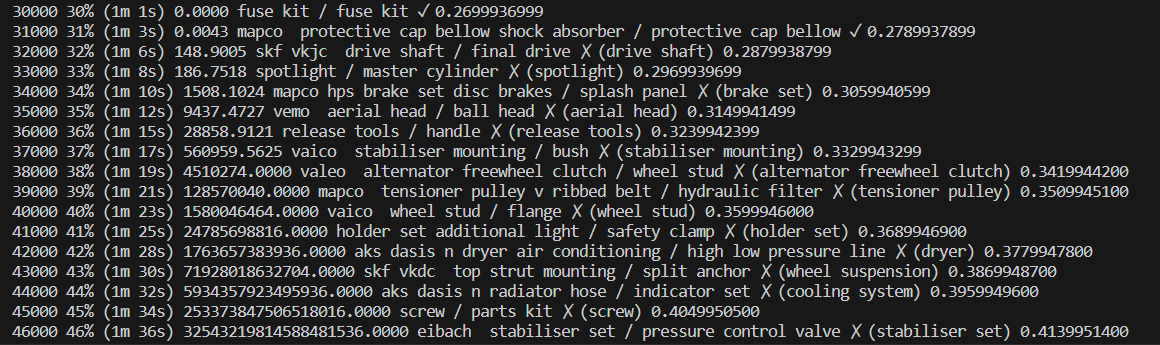
\includegraphics[scale=0.6]{loss_nan.png}
        \caption{Result: Loss value returning nan}
        \label{fig:Loss value}
    \end{figure}


    \item In the next experiment, we set the $max\_lr = 0.2$. \\
    The classification model successfully completed the training and was able to predict the category.
    \begin{figure}
        \centering    
        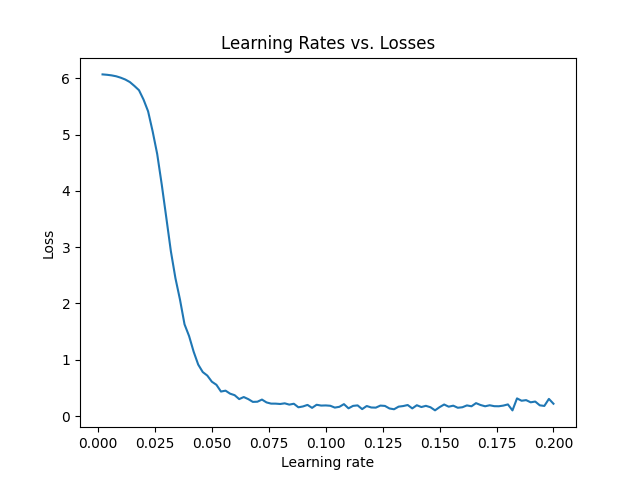
\includegraphics[scale=0.8]{loss_lr_02.png}
        \caption{Loss vs Learning rate; where $max\_lr = 0.2$}
        \label{fig:Loss value at 0.2}
    \end{figure}
    
    As illustrated in figure \ref{fig:Loss value at 0.2}, in the graph plotted of Loss Vs Learning rate. The model started to learn at learning rate $\epsilon = 0.04$ onwards. We will further reduce the $max\_lr$.

    \item In the next experiment, we set the $max\_lr = 0.04$. \\
    Notice in figure \ref{fig:Loss value at 0.04}, there is a plateau until $\epsilon = 0.010$. After which there is a descent until $\epsilon = 0.015$
    \begin{figure}
        \centering    
        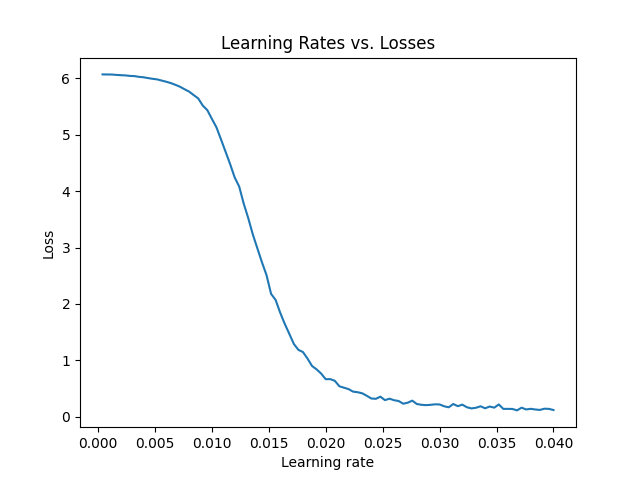
\includegraphics[scale=0.9]{loss_004.png}
        \caption{Loss vs Learning rate; where $max\_lr = 0.04$}
        \label{fig:Loss value at 0.04}
    \end{figure}

    \item In the next experiment, we set the $max\_lr = 0.015$. \\
    Notice in figure \ref{fig:Loss value at 0.015}, the loss had not neared zero and the model fails to predict the classification. 
    \begin{figure}
        \centering    
        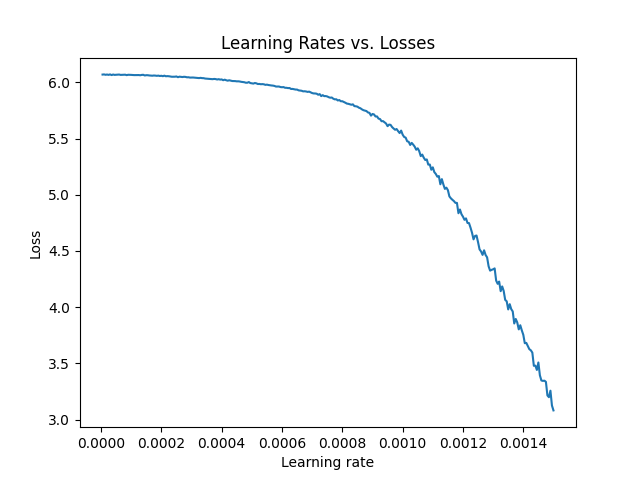
\includegraphics[scale=0.9]{loss_0015.png}
        \caption{Loss vs Learning rate; where $max\_lr = 0.015$}
        \label{fig:Loss value at 0.015}
    \end{figure}

    \item From the earlier mentioned experimentation with $max\_lr$,  the loss in classification model is nearing zero by the end the training  when  $max\_lr > 0.015$ 
    Figure \ref{fig:Loss value at 0.02} illustrates the loss reaching near zero when $max\_lr = 0.02$. The figure  \ref{fig:Loss value at 0.02}, there is a plateau until the $ \epsilon = 0.0075$. Indicating that the model did not learn until the learning rate $ \epsilon = 0.0075$.
    \begin{figure}
        \centering    
        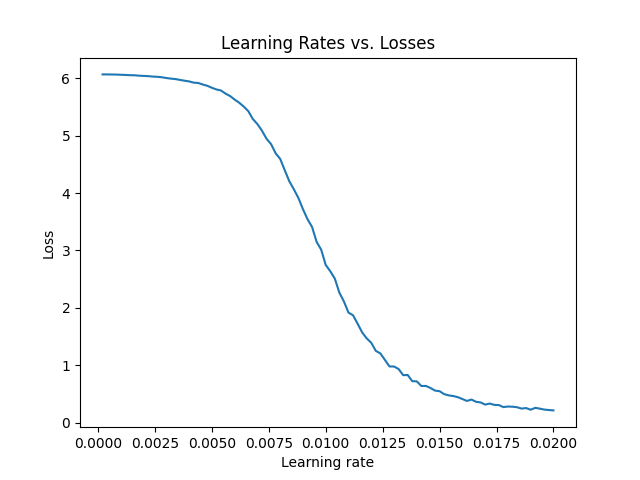
\includegraphics[scale=0.9]{loss_002.png}
        \caption{Loss vs Learning rate; where $max\_lr = 0.02$}
        \label{fig:Loss value at 0.02}
    \end{figure}

    \item Updating the $base_lr=0.0075$ and $max_lr=0.02$, resulted a steady slop in the loss vs learning rate.  
    Figure \ref{fig:Loss value at 0.0075} illustrates the loss reaching near zero when $max\_lr = 0.02$ and $base_lr=0.0075$. The steady decent indicates the learning rate range is optimal.
    \begin{figure}
        \centering    
        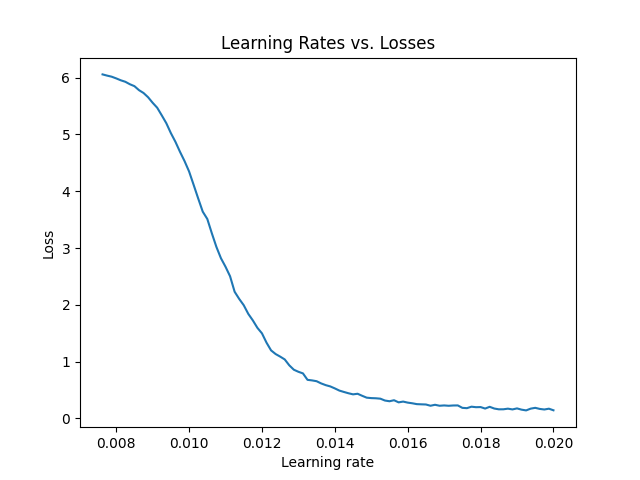
\includegraphics[scale=0.9]{loss_0075_002.png}
        \caption{Loss vs Learning rate; where $base\_lr = 0.0075$ and $max\_lr = 0.02$ }
        \label{fig:Loss value at 0.0075}
    \end{figure}
    

\end{enumerate}

\section{Triangular learning rate}

\parencite{Smith.03062015} introduced the concept of letting the learning rate vary within the range of minimum and maximum boundaries of learning rate known as learning rate range. In this method the learning rate linearly increases until step size $ t $ and then linearly decreases. 


How triangular learning rate works?
\begin{enumerate}
    \item \textbf{Initialize}: The step size $ t $, minimum bound or base learning rate $ base\_lr$ and maximum bound or the max learning rate  $max\_lr$ are initialized. These hyperparameters are tuned based on the architecture of the model. In this experiment, the values set are  $ base\_lr=0.0075 ; max\_lr=0.02; t=10000$.
    \item  \textbf{Up phase}: During training, the learning rate is linearly increased from $ base\_lr$ to $max\_lr$ over a certain number of step size $ t $.
    \item \textbf{Down phase}: During training, the learning rate is linearly decreased from $max\_lr$ to $base\_lr$.
\end{enumerate}

\begin{figure}[H]
    \centering    
    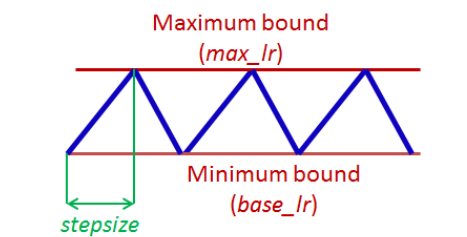
\includegraphics[scale=0.9]{triangular learning rate.png}
    \caption{Triangular learning rate policy.  \parencite{Smith.03062015}
    }
    \label{fig:trl}
\end{figure}
 Figure \ref{fig:trl} is pictorial representation of triangular learning rate. The blue lines represent learning rate values changing between the bounds. The input parameter step-size is the number of iterations in half a cycle \parencite{Smith.03062015}.

 \begin{lstlisting}[language=Python,label={code:triangularLR}, caption={Triangular learning rate}]
def runBatchWithTLR(self):
# each unit is half cycle iteration 
    batch=[10000,10000,10000,10000,10000,10000,10000,10000,10000,10000]        
    start = time.time()
    no_batch=0
    no_iterations=0
    learning_rates =[]

    for n_iters in batch:

        no_batch =no_batch+1
        rem=no_batch % 2
        # linearly space the learning rate by number of iterations using np.linspace
        learn_rates=np.linspace(self.lr_low,self.lr_max,n_iters)
        # for even number of batch flip the array for down phase
        if rem==0:
            learn_rates=np.flip(learn_rates)
        
        # run the iterations along with the linearly spaced learning rate.
        for epoch,lr in zip(range(1, n_iters + 1),learn_rates):
            no_iterations= no_iterations+1
    
            self.learning_rate=lr              
            category, name, category_tensor, name_tensor = self.data.randomTrainingExample()
            
            output, loss = self.train(category_tensor, name_tensor)
            self.current_loss += loss
            # Print ``iter`` number, loss, name and guess
            if epoch % 5000 == 0:
                guess, guess_i = self.data.categoryFromOutput(output)
                correct = 'yes' if guess == category else 'no (%s)' % category
            
                print('%d %d%% (%s) %.4f %s / %s %s %.10f' % (no_iterations, 
                                            no_iterations / np.sum(batch) * 100,
                                            self.helper.timeSince(start),
                                            loss,
                                            name, 
                                            guess, 
                                            correct, self.learning_rate))

         
            if epoch % 5000 == 0:
                if (math.isnan(self.current_loss)!=True):
                    self.all_losses.append(self.current_loss / 5000)
                    learning_rates.append(self.learning_rate)
                    self.current_loss = 0
                else:
                    break
\end{lstlisting}

Listing \ref{code:triangularLR} is the code to train the model using triangular learning rate. Below is the explanation of the code.

\begin{enumerate}
    \item \textbf{Variable initialization}: 
    \begin{itemize}
        \item \textbf{batch}: \\ A list of elements representing number of iterations in a batch. Each batch represents half cycle or step-size.
        \item \textbf{start = time.time()} :\\ This stores current time at the beginning of the training process.
    \end{itemize}
    \item Batch iteration: \\
     \begin{itemize}
        \item \textbf{rem = no\_batch \% 2}: \\ Calculates reminder of no\_batch. It determines whether to flip the learning rates array. If rem is 0 (indicating an even batch number), the array is fliped using numpy's \parencite{harris2020array} \textit{np.flip} method.
        \item learn\_rates :\\ This stores linearly spaced learning rates between $base\_lr$ and $max\_lr$ divided into batch size.
    \end{itemize}
    
    
\end{enumerate}


\subsection{Experimentation and analysis}
In this experiment, the model is trained with and without triangular learning rate method. The total number of iterations is $10000 \times 10$. The graph of Loss Vs Learning rate and time taken to complete the iterations illustrates the performance of the model. The graph plotted for each $2500$ iterations provide insight on how the model is performing. 
\begin{enumerate}
    \item Triangular learning rate; where $base\_lr =0.0075$ and $max\_lr=0.02$: \\
    
    \begin{figure}[H]
        \centering    
        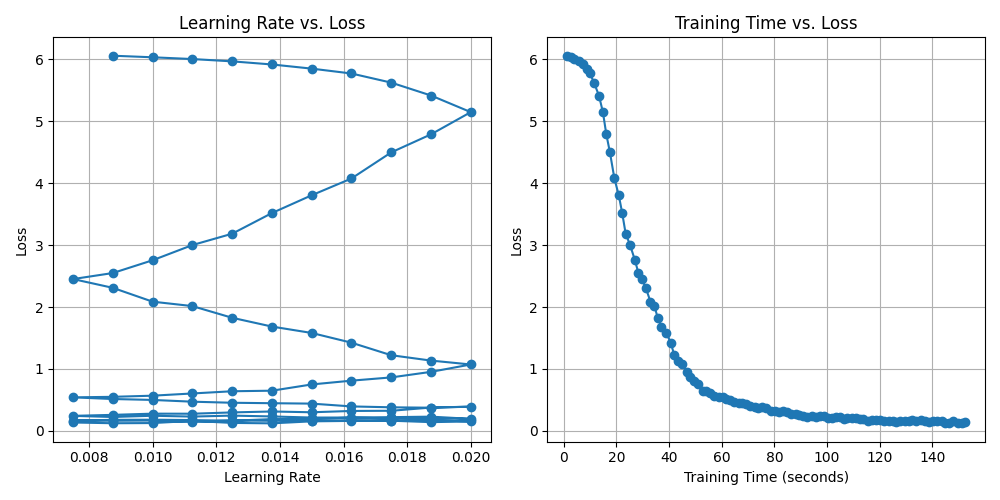
\includegraphics[scale=0.5]{lossinfo_tlr.png}
        \caption{Loss with TLR, where $base\_lr =0.0075$ and $max\_lr=0.02$
        }
        \label{fig:trl_loss}
    \end{figure}

   
    
\end{enumerate}

\section{Model Evaluation}

The model is evaluated using the confusion matrix. Confusion matrix is square matrix of predicted label $y_{pred}$ verses the true target label $y_{true}$.
Figure \ref{fig:meval} is the confusion matrix of the model trained only for 20 categories. The actual model is trained to predict around 300 categories. Author choose to attach the miniature version of the confusion matrix.  Refer Appendix A code \ref{code:confusion matrix} for the python code to generate a confusion matrix.

\begin{figure}[H]
    \centering    
    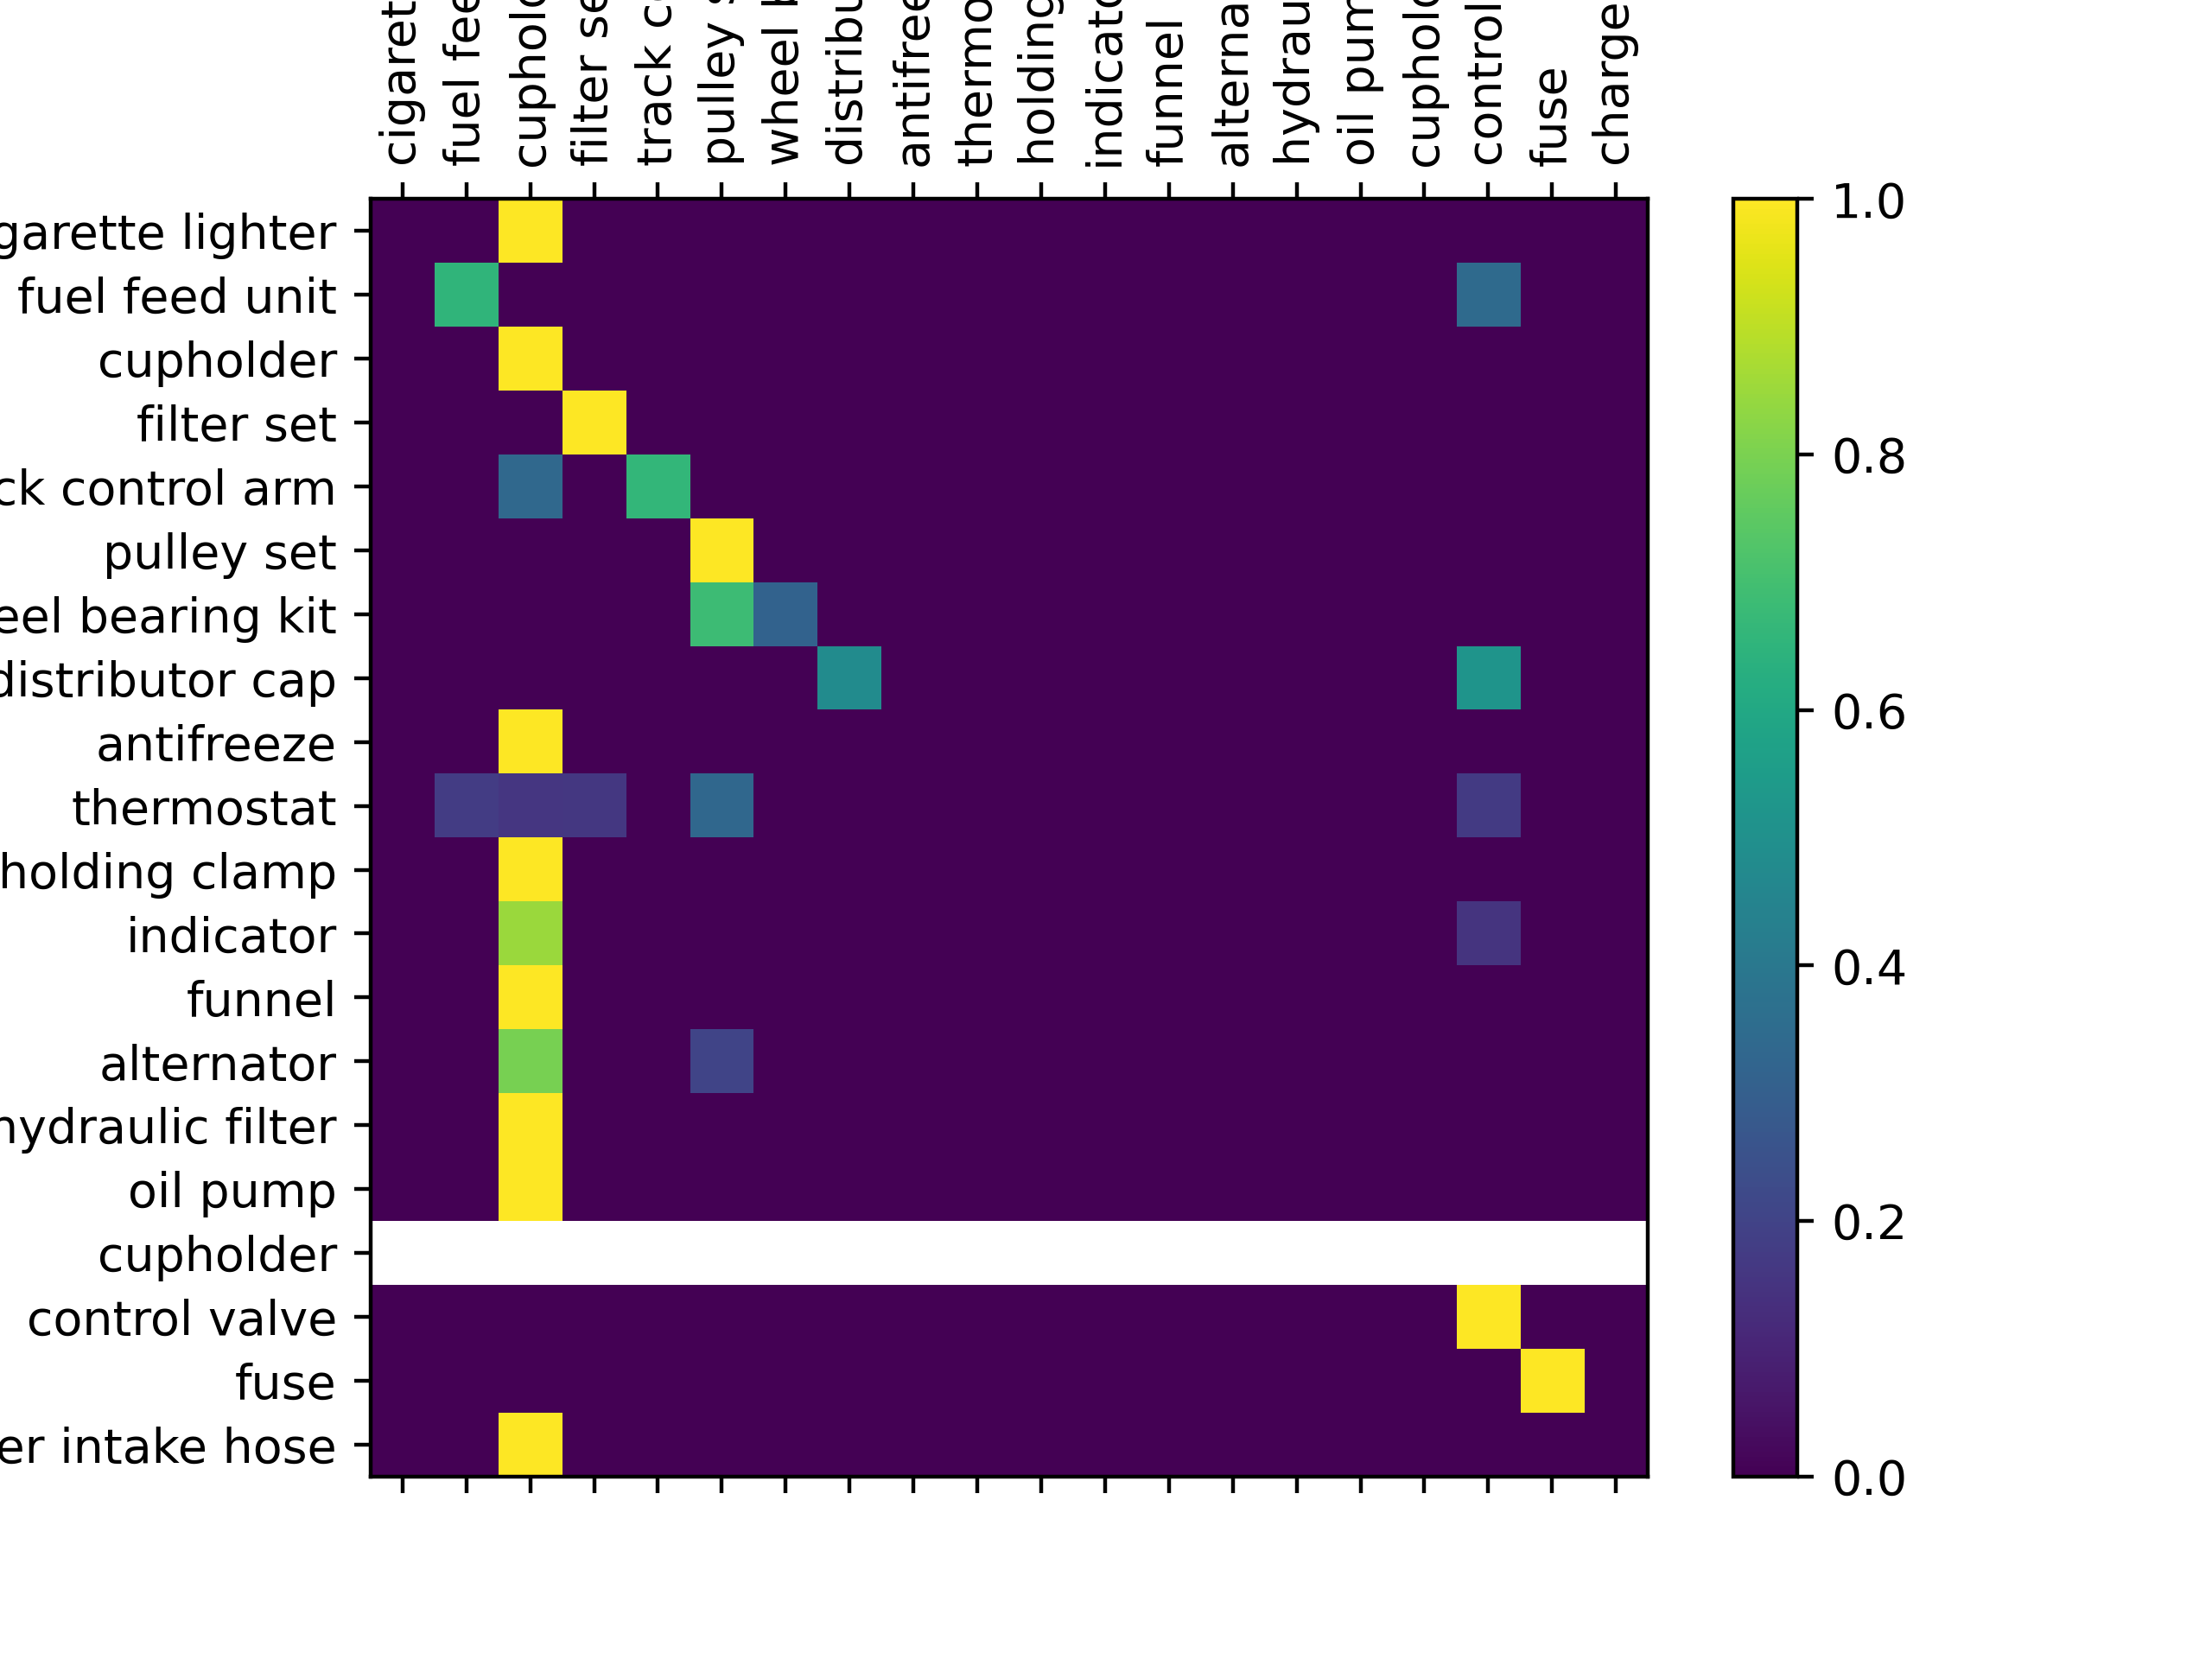
\includegraphics[scale=0.5]{confusion._200epoch.png}
    \caption{Confusion matrix: with little training.
    }
    \label{fig:meval}
\end{figure}

\subsection*{Actual vs Predicted category}
Author tested the model with test data of 10000 pairs of product name and category.
Analyzing the falsely predicted result of 1455 records gained insight of incorrect categorization of existing products.  Table \ref{table:false_negative} refers to a sample of record which the model falsely predicted the category.\\ Which means  $y_{pred} \neq y_{true}$. However, this records indicate a false negative record, which means the $y_{pred}$ is incorrectly saved possibly due to human error. 

     
\begin{table}[h]
    \centering
    \caption{False negative - sample data}
    \label{table:false_negative}
    \begin{tabular}{ lll }
          \toprule
          
          \textbf{Name} & \textbf{$y_{true}$} & \textbf{$y_{pred}$} \\
          \midrule
          RPM Sensor, engine management&Sensor&RPM Sensor \\
        
          \bottomrule
          \end{tabular}
\end{table}

\section{Model Deployment}

A \textbf{.pt} file represents the PyTorch model checkpoint file. These files store the parameter and architecture of trained PyTorch model. The PyTorch's torch.save and torch.load function uses the pythons  Pickle (refer section \ref{sec:ngram_vector}) utility for serialization \parencite{savept}.

As the \acl{PIM} systems get updated with the latest details of product information, the model requires retraining for accurate prediction. Refer Appendix A code \ref{code:Loadpt} for Python code to load the trained PyTorch model.

\section{Summary}

This chapter is about the result of classification model. How the normalized text data is indexed and fetched from the elastic search is mentioned in this chapter. Initialization of the Train class and its input parameters detailed explanation is given in this chapter.  

What is \acf*{BPTT}? How its relevant backwards methods works? are mentioned in the chapter.

Author experiments with the model parameters and evaluates the model based on the logarithmic loss value. 

Few training experiments are:
\begin{itemize}
    \item Training model without any learning parameters.
    \item Updating the number of hidden states in a neural network.
    \item Determining the learning rate range.
    \item Training with Triangular learning rate.
\end{itemize}


This chapter also describes the gradient decent \parencite{cauchy} step adjustment and compares the equation with the Pytorchs's tensor gradient method of adjustment with learning rate.  